\subsection{Learned conditional densities with explicit tail structure}
We train five mixture density networks on joint samples from a two-mode simulator, using conditional negative log likelihood and no exact-posterior labels. Each network completes 40,000 updates. Its output is a two-component Gaussian mixture with a shared, bounded component variance, so the noised score is exact conditional on the learned parameters. This architecture makes tail curvature available to the certificate. Five dataset seeds crossed with the five checkpoints give 25 pairs for each $(G,d)$ configuration. We compare particles with both the learned composition and the true posterior, using $P=32768$, $M=4$ and $K\in\{512,2048\}$; Appendix~\ref{app:extension-protocol} gives the simulator, training checks and complete protocol.

All 1,000 learned sampling cells pass independent raw-sample, reference-density and certificate audits. Full weighting and both tail controls have finite population normalizers in all 600 corresponding cells; both raw unbiased estimators have infinite normalizers in all 400 remaining cells. Without replacement therefore does not restore validity at this batch size. Across the four $(G,d)$ settings, mean W1 between the true and learned compositions ranges from $0.00536$ to $0.00801$, and mean KL from $0.00075$ to $0.00304$.

\begin{figure}[t]
 \centering
 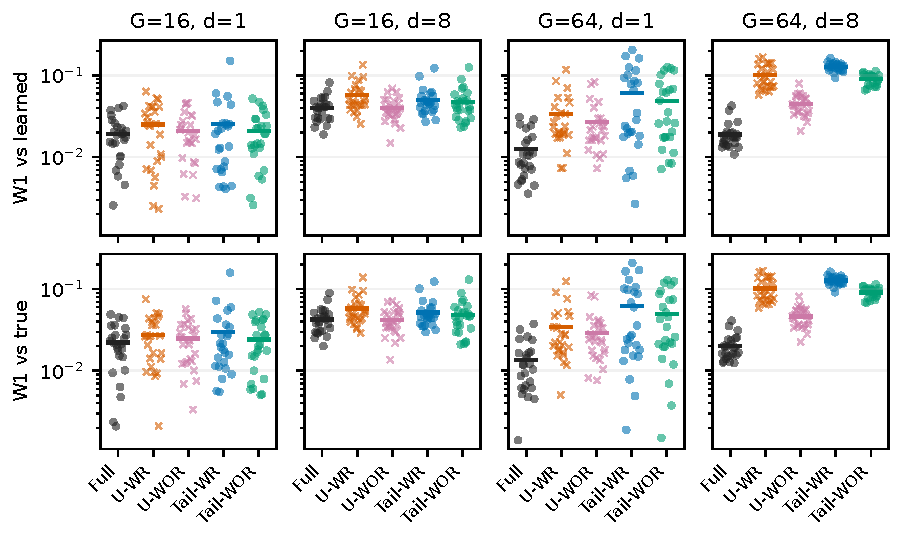
\includegraphics[width=\linewidth]{figures/learned_results.pdf}
 \caption{Learned-posterior sampling at the preselected $K=2048$. Each panel shows all 25 crossed checkpoint/dataset pairs; horizontal bars are means. Circles denote finite population normalizers and crosses infinite ones. U is raw unbiased weighting; WR and WOR denote sampling with and without replacement. The upper row measures particle W1 against the learned composition and the lower row against the true posterior. These 25 pairs are not independent training replicates.}
 \label{fig:learned}
\end{figure}

Figure~\ref{fig:learned} again separates validity from accuracy. At $G=64,d=8,K=2048$, W1 against the learned composition is $0.0189\pm0.0073$ for full weighting, $0.0448\pm0.0130$ for raw without-replacement weighting, and $0.0907\pm0.0136$ for tail control without replacement. Against the true posterior, the corresponding values are $0.0201$, $0.0462$ and $0.0912$. Tail control restores the finite domain but has larger errors in this comparison. Its recorded mean sampler time is 5.73 seconds, versus 26.09 seconds for full weighting; at $G=16,d=1$, it instead takes 3.86 seconds versus 2.27 seconds. These timings include subset selection and exclude separately recorded one-time neural parameter prediction. They provide no universal accuracy or speed advantage, and do not measure repeated neural score evaluations.
